\section{implementation}
\begin{figure*}[ht]
  \centering
  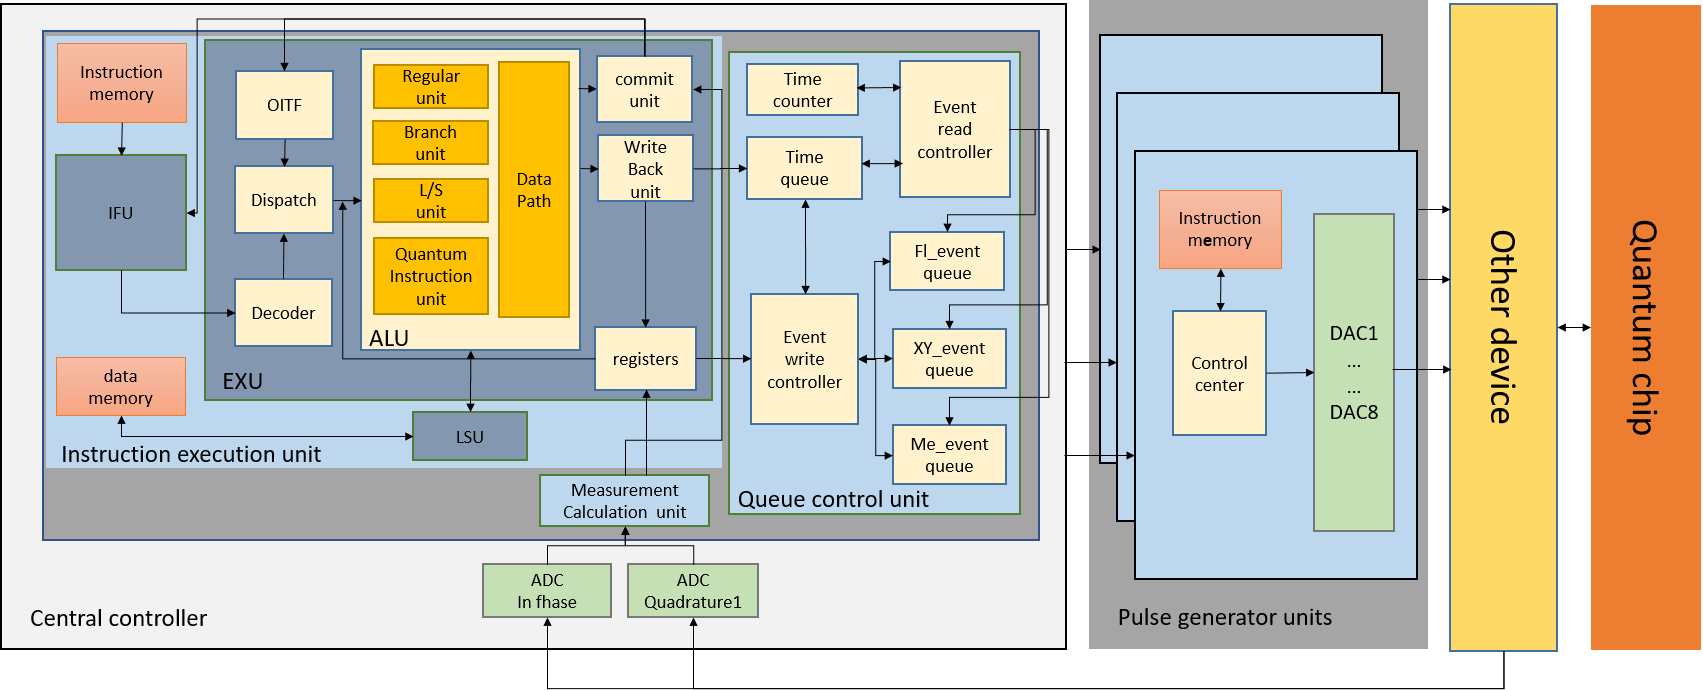
\includegraphics[width=\linewidth]{figure/5_1}
  \caption{overview of electrode event-based microarchitecture}
  \label{img7}
\end{figure*}
In this Section, we discuss the implementation of ebQuMA. ebQuMA consists of a central controller and multiple waveform generation units, 
as shown in Figure 10. The central controller is implemented using an Arrow BeMicroCV A9 board holding an Altera Cyclone V 5CEFA9 FPGA chip, 
connects to two 8-bit resolution analog-to-digital converters (ADC) to digitize analog measurement signals. 
The central controller consists of instruction execution unit, queue control unit, and measurement calculation unit. 
The clock frequency of the instruction execution unit is 100MHz, and 50MHz for Queue control unit.

The instruction execution unit is a two-stage pipelined processor architecture. 
Since the encoding format of quantum instructions in ebQIS is the same as the classical instruction, 
they are executed at the same stage. The instruction fetch unit (IFU) reads the instruction from the instruction memory and sends it to the execution unit (EXU). 
The Exu decodes and checks the data and resource correlation through the outstanding instruction track fifo (OITF). If there is a conflict, the pipeline is blocked. 
In addition to the classic WAW, WAR, and RAW conflicts, when the dispatched instruction is FMR or Measure but the last measurement result of the target qubit is not returned, 
a conflict also occurs, until the measurement result is returned. At the same time, when instructions are dispatched, 
the entries of potentially conflicting instructions are stored in the OITF, 
Such as target qubit of measure instruction and the destination register index of Load instruction.
If there is no conflict, the dispatch module will send it to one of the four unit of the arithmetic and logic unit according to the instruction type, 
which are used to perform arithmetic logic operations, branch instructions, storage instructions and quantum instructions respectively, 
and reuse the same data path for calculation.

Here, we only introduce the execution process of quantum instructions.
If the PI of the quantum instruction is 0, the electrode event coding of up to two quantum operations in the current 
instruction are added to the value of the event register of target qubit (for XY feedline local event) or the global event register (for flux bias line event). 
For the global event of XY feedline, the XY feedline event register for each qubit is added to the event coding. 
The event register is used to buffer the event of each electrode with the same timestamp. 
If PI is not zero, the event of the current instruction is written to the corresponding event register, 
and rest of event registers are set to zero. At the same time, a new timestamp is calculated by data path. 
As for the Qwait, FMR, and SMIS instructions, the execution method is similar to the ADD instruction, except that the source and destination registers are different. 

The write back unit (WBU) update registers with the calculation results from ALU. 
If the current instruction generates a new timestamp, the WBU sends the value of all event registers to the queue control module, 
as well as the new timestamp. The commit unit is responsible for pipeline flushing and update of entries in the OITF. 
After complete the write back of Load instruction or measurement instruction, the entries in the OITF are cleared by the commit unit. 
The LSU module is used for data interaction with the data memory.

The queue control unit realizes precise time control of the quantum processor. The queue writing controller buffers the timestamp and event sent by the instruction execution unit to the corresponding electrode event queue and time queue. 
When a trigger signal is received, the time counter starts counting. If the counter is equal to the head element of the time queue, the electrode events corresponding to this timestamp are sent to the pulse generator units by the event read controller. 

In particular, when there is only one element left in the time queue and the value of the time counter is equal to it, 
To prevent timing errors, the time counter will suspend counting until a new timestamp is received. At the same time, 
the event read controller sends the accepted electrode event (event corresponding to the last timestamp in time queue) directly to the pulse generator unit through the bypass.
This situation occurs when the instruction execution module needs to execute more instructions to obtain electrode events at the next point in time, 
so that all buffered events have been executed, mainly in feedback programs based on measurement results.

Although this scheme will cause the applied waveform not to strictly follow the timing specified by the instruction, 
in fact, for quantum applications, it is only necessary to ensure that the execution time interval of two quantum gates is not less than the duration time of the first quantum gate to avoid error.
For the circuit that need to be executed strictly in accordance with timing, 
such as calibration experiments, high-level abstraction of electrode event can be used. 
Since the instruction execution time is much shorter than the waveform length, this situation will not occur.

The measurement calculation unit (MCU) analyzes and processes the measurement waveforms of the qubits collected by the ADCs to obtain the states of target qubits. 
For more detail about measurement discrimination using a customized FPGA, please refer to []. 
When the qubit status is obtained, the MCU updates the qubit measurement result register and submits an application for measurement completion to the commit unit.
